\Chapter{MAGNIS (MAGnetized Negative Ion Source)}
\begin{refsection}

\chaptermark{Modèles plasmas froids magnétisés}

Dans ce chapitre, nous proposons un nouveau modèle fluide pour décrire le
transport magnétisé dans les plasmas froids. Nous discutons tout d'abord de
l'approche standard de modélisation des plasmas froids, des problématiques qui
lui sont propres ainsi que des difficultés rencontrées lors du développement du
modèle basé sur les vitesses de dérive. La suite concerne l'élaboration du
nouveau modèle, nous le dérivons en expliquant les différents termes essentiels
à description du transport dans les plasmas froids puis nous détaillons le
schéma numérique original utilisé pour résoudre les équations.
Une dernière partie est consacrée à la vérification du code par une étude de
convergence sur maillage et à une validatation élémentaire du comportement du
plasma dans des cas théoriques représentatifs.



\section{Problématique}

La compréhension de l'origine et de la nature du transport dans les plasmas
magnétisés est un enjeu majeur pour la conception, la réalisation et
l'optimisation de nombreuses applications et procédés. Dans les sources plasmas
fonctionnant à basse pression,  La plupart des modèles fluides décrivant les
phénomènes de transport magnétisés dans les plasmas froids sont basés sur les équations de dérive-diffusion (\S \ref{1-deriveDiffMag}). Cependant, au delà d'une certaine intensité de champ magnétique, l'anisotropie du transport rend la résolution numérique de ces
équations complexe voire impossible\footnote{Le problème est alors généralement
adressé à travers le développement de modèles cinétiques numériquement très
coûteux, et nécessitant à priori la résolution d'échelles de l'ordre de la
longueur de Debye et de la fréquence plasma.}.
Celles-ci sont en fait peu adaptées au transport fortement
magnétisé~\cite{Golant}.

L'un des points délicats dans la modélisation du transport magnétisé concerne la
discrétisation de l'équation du mouvement. Au fur et à mesure de l'augmentation
du champ magnétique, les flux magnétisés dominent de plus en plus sur les termes
collisionnels.

Un indice nous est donné en considérant la description du transport transverse
par les vitesses de dérive (cf.
introduction) où l'équilibre des courants fait intervenir la divergence de la
dérive de polarisation. Cette dérive, essentielle dans la dynamique du transport
transverse, est absente du modèle qui néglige totalement l'inertie des
particules. Le modèle de dérive-diffusion cherche une solution stationnaire à un
problème intrinsèquement non-stationnaire.
\parencite{Fruchtman}
\parencite{Sternberg}
D'un autre côté,

\section{Description du modèle}
Le plasma est constitué d'électrons et d'une ou plusieurs espèces d'ions de
charge $q_\alpha$ et de masse $m_\alpha$. On considère un plasma de taille $L$,
confiné et en interaction avec des parois à travers une gaine large de quelques longueurs
de Debye. La longueur $L$ est prise suffisement grande $L\gg\lambda_D$ pour
supposer le plasma quasi-neutre. Le champ magnétique $\mathbf{B}$ imposé est 
stationnaire, de sorte que le champ électrique dérive directement d'un 
potentiel électrostatique $\mathbf{E}=-\nabla \Phi$. Le transport est décrit
dans le plan perpendiculaire au champ magnétique et les conditions aux limites
parallèles, qui dérivent d'une théorie classique de gaine, sont
inclues directement dans les équations de conservation à travers des termes
sources.

\subsection{Equations de conservation}
Pour décrire l'évolution des espèces dans un plasma partiellement ionisé, basse
pression et magnétisé, l'équation du mouvement doit tenir compte de
l'interaction avec le gaz, de l'inertie et du terme de Laplace :

\begin{equation}
\partial_t \mathbf{u}_\alpha + \mathbf{u}_\alpha\cdot\nabla\mathbf{u}_\alpha+
\nu_\alpha\mathbf{u}_\alpha+\omega_{c\alpha}\mathbf{b}\times\mathbf{u}_\alpha=
-\frac{q_\alpha}{m_\alpha}\left(\nabla \Phi+\frac{\nabla
p_\alpha}{q_\alpha n_\alpha}\right)
\end{equation}

où $n_\alpha$ est la densité de l'espèce considérée, $\mathbf{u}_\alpha$ sa
vitesse fluide, $p_\alpha =en_\alpha T_\alpha$ la pression (dont nous ne
retenons que la contribution isotrope) et $\Phi$ le potentiel électrostatique. La fréquence
cyclotronique est notée $\omega_{c\alpha}=q_\alpha B/m_\alpha$ et $\nu_\alpha$
est une fréquence effective rendant compte des collisions.
Le transfert de quantité de mouvement dû aux collisions contient la perte liée à
l'ionization
$\nu_\alpha=\nu_{\alpha}^\text{iz}+\nu_{\alpha}^{c}+\nu_{\alpha}^{ei}$ où
$\nu_{\alpha}^{c}$ et $\nu_{\alpha}^{ei}$ sont respectivement les
fréquences de collisions particules chargées - neutres et de collisions
coulombiennes.

L'évolution de chaque espèce est décrite par une équation de continuité :

\begin{equation}
\label{3-continuite}
\partial_t n_\alpha +
\nabla\cdot\left(n_\alpha\mathbf{u}_\alpha\right)=S_\alpha(T_e)
\end{equation}

avec $S_\alpha$ un terme d'ionisation, fortement dépendant de la
température électronique $T_e$. En considérant l'hypothèse de quasi-neutralité, la somme des
équations de continuité conduit à l'équation de conservation du courant :

\begin{equation}
\label{eqCourant}
\nabla\cdot(\sum_ien_i\mathbf{u}_i-en_e\mathbf{u}_e)=0
\end{equation}

où l'indice i dénote éventuellement différentes espèces d'ions. 
L'équation \eqref{eqCourant} couple les différentes espèces en contrôlant
l'évolution du potentiel électrostatique $\Phi$.

L'équation de conservation de l'énergie est obtenue classiquement en substituant
l'équation de continuité afin d'éliminer le terme convectif :

\begin{equation}\begin{split}
\label{3-energie}
\frac{3}{2}en_e\partial_tT_e + \nabla\cdot(\mathbf{q_e}) +
(\frac{5}{2}S_e-\partial_tn_e)eT_e \\=n_e\mathbf{u}_e\cdot(\nabla
\Phi-\frac{5}{2}e\nabla T_e)+n_e\left(P_{ext}-\Pi\right)
\end{split}
\end{equation}

où $T_e$ est la température électronique exprimée en eV, $S_e$ est le
terme source d'électrons lié à l'ionisation, $P_\text{ext}$ la puissance
extérieure déposée dans le plasma et $\Pi$ le terme de perte d'énergie dûe aux
collisions. La fermeture du modèle se fait alors sur le flux de chaleur
$\mathbf{q}_e$, tel qu'exprimé par
V.E. Golant dans~\cite{Golant} :

\begin{equation}
\partial_t \mathbf{q}_e + \nu_e\mathbf{q}_e+\omega_e\mathbf{q}_e\times\mathbf{b} =
-\frac{5}{2}\frac{e^2}{m_e}n_eT_e\nabla T_e
\end{equation}

Le flux de chaleur est magnétisé de la même façon que le flux de matière et
dépend essentiellement du gradient de température. Dans les sources magnétisées,
où la longueur de gradient thermique est de l'ordre de la largueur
du filtre magnétique, le flux de chaleur influence fortement le transport
transverse. Il doit donc nécessairement être pris en compte et décrit
avec le minimum d'approximations.

\subsection{Conditions aux limites}
Le modèle quasineutre est complété par la
définition des conditions aux limites portant sur les flux et intégrant le
maximum de considérations physiques. Dans le cas d'une paroi conductrice, un
modèle classique de gaine non-collisionnelle est utilisé. Les flux ioniques et
le flux électronique sont définis en l'entrée de gaine par :

\begin{align}
&\Gamma_i=n_i\mathbf{u}_i\cdot\mathbf{n}=n_i.\max\left(c_s,\mathbf{u_i}\cdot\mathbf{n}\right)
\\
&\Gamma_e=n_e\mathbf{u}_e\cdot\mathbf{n}=n_e\frac{1}{2\sqrt{\pi}}v_{Te}=n_ec_s\exp(\Lambda-\Delta
\Phi/T_e)
\end{align}

avec $\mathbf{n}$ le vecteur normal à la paroi,
et $c_s=(eT_e/m_i)^{\text{\textonehalf}}$ la vitesse acoustique ionique. Le flux
d'électron est obtenu en considérant une fonction de distribution maxwellienne, 
que l'on intègre sur le demi-espace des vitesses dirigées vers la paroi avec 
$v_{Te}=(2eT_e/m_e)^{\text{\textonehalf}}$ la vitesse électronique thermique.
$\Delta\Phi$ la différence entre le potentiel plasma $\Phi$ et le potentiel de
la paroi $\Phi_w$ se réécrit pour un courant nul:

\begin{equation}
	\mathbf{j}\cdot\mathbf{n}=0\Leftrightarrow \Delta \Phi=\Phi-\Phi_w =
T_e(\Lambda-ln\sum_i\mathbf u_i/c_s)
\end{equation} 

où le potentiel flottant $\Lambda$ est défini pour un plasma
n'étant composé que d'une espèce :

\begin{equation}
	\Lambda=ln\left(\frac{eT_e}{2\pi
	m_e\mathbf{u}_i^2}\right)^{\text{\textonehalf}} \le 
	ln\left(\frac{m_i}{2\pi m_e}\right)^{\text{\textonehalf}}
\end{equation}

Les ions sont perdus au minimum avec la vitesse acoustique, mais
éventuellement avec une vitesse supersonique. Le flux d'électron s'ajuste
quant à lui pour réguler potentiel autour de sa valeur
d'équilibre définie par le potentiel flottant $\Phi=\Lambda T_e$. La condition
limite pour le courant est par conséquence définie par :

\begin{equation}
\Gamma_j=\mathbf{j}\cdot\mathbf{n}=e\sum_in_i{\mathbf
u}_i-en_ec_s\exp(\Lambda-\Delta \Phi/T_e)
\end{equation}

Si la paroi est isolante, la surface se polarise pour assurer la nullité du
courant sortant :

\begin{equation}\begin{split}
\mathbf j\cdot\mathbf{n}=0\Leftrightarrow
\Phi_w=\Phi-T_e(\Lambda-ln\sum_i\mathbf u_i/c_s)
\end{split}\end{equation}

L'énergie perdue par les électrons en entrée de gaine s'obtient en
additionnant l'énergie moyenne perdue à la paroi (intégrée sur une distribution
semi-maxwellienne) et l'énergie transférée aux ions dans la chute de potentiel :

\begin{equation}
	\varepsilon_w=2T_e+\Delta \Phi
\end{equation}
 
 On peut alors relier cette perte totale aux flux sortants de l'équation
 d'énergie \eqrefp{3-energie}, qui correspondent au flux d'énergie porté par
 les particules et au flux de chaleur :
 
\begin{equation}
\Gamma_\varepsilon=\frac{5}{2}{\Gamma}_eT_e+\mathbf{q}_e\cdot\mathbf{n}=
\Gamma_e\left(2T_e+\Delta \Phi\right)
\end{equation}

En regroupant les termes portant sur le flux d'électron, on peut exprimer la
condition limite pour le flux de chaleur :

\begin{equation}
\mathbf{q}_e\cdot\mathbf{n}=\Gamma_e\left(\Delta \Phi-\frac{1}{2}T_e\right)
\end{equation}

Ces conditions aux limites sont justifiées dans des plasmas non-magnétisés et à
l'extrémité de lignes de champ interceptant la paroi dans
des plasmas magnétisés. Dans la direction perpendiculaire au champ magnétique,
nous gardons comme hypothèse que le la vitesse ionique doit au
minimum atteindre la vitesse de Bohm pour permettre une brisure de
la quasineutralité du plasma et l'apparition d'une gaine de charge d'espace
positive.

\subsection{Réduction 2D du modèle}
Le système d'équations Eqs.(\ref{3-continuite}~-~\ref{3-energie}) décrit le
transport magnétisé dans un plasma froid en suivant l'évolution des densités de
particules $n_\alpha$, du potentiel électrique $\Phi$ et de la température
électronique $T_e$ dans un espace à trois dimensions. 

Le champ magnétique n'affecte que très peu les particules dans la direction
parallèle aux lignes de champ : le plasma est stationnaire, et les électrons, en
équilibre de Boltzmann le long des lignes, permettent le transport rapide des fluctuations des quantités
macroscopiques électroniques dans la direction parallèle. Le problème du
transport magnétisé se réduit alors essentiellement au problème du transport
dans plan perpendiculaire à $\mathbf B$, qui est le plan des dérives et des
fort gradients.

La dissociation des mouvements parallèle et perpendiculaire s'effectue
en réécrivant les équations dans un repère axé sur le champ magnétique
(O,$\mathbf x$,$\mathbf y$,$\mathbf b$), puis nous refermons le
système en l'intégrant le long de la direction parallèle. Les conditions aux
limites au bout des lignes de champ apparaissent ainsi comme des termes source
ou perte dans les équations de conservation :

\begin{align}
\label{3-vitessesBord}
\begin{split}
\Gamma&_{i_\para}=\frac{1}{L_\para}\int_{-L_\para/2}^{L_\para/2}\nabla_\para\left(n_iu_{i_\para}\right)=\frac{2a}{L_\para}n_ic_s\\
\Gamma&_{e_\para}=\frac{1}{L_\para}\int_{-L_\para/2}^{L_\para/2}\nabla_\para\left(n_eu_{e_\para}\right)=\frac{2}{L_\para}n_ec_s
\exp(\Lambda-\Delta \Phi/T_e)\\
\Gamma&_{j_\para}=\frac{1}{L_\para}\int_{-L_\para/2}^{L_\para/2}\nabla_\para\left(j_\para\right)=\sum_i\Gamma_{i_\para}-\Gamma_{e_\para}\\
\Gamma&_{\varepsilon_\para}=\frac{1}{L_\para}
\int_{-L_\para/2}^{L_\para/2}\nabla_\para
\left(\frac{5}{2}n_eT_eu_{e_\para}+q_{e_\para}\right)
=\frac{2}{L_\para}n_eu_{e_\para}(2T_e+\Delta \Phi)
\end{split}
\end{align}

où $L_\para$ est la taille du plasma dans la direction du champ magnétique. Pour
les électrons, $\Gamma_{e_\para}$ implique le potentiel de la paroi au bout des
lignes de champ. Pour les pertes ioniques, un facteur $a$ représente le ratio
entre la densité de particules à l'entrée de la gaine et la densité moyenne
calculée le long des lignes de champ. Après cette opération de fermeture,
le système d'équation peut se réécrire en fonction des variables moyennées
($\bar{n}_\alpha$, $\bar{\mathbf u}_\alpha$,$\bar{T}_e$\ldots) :

\begin{align}
\label{3-equations2D1}
\partial_t \bar{n}_\alpha& +
\nabla_\perp\cdot\left(\bar{n}_\alpha\bar{\mathbf{u}}_{\alpha_\perp}\right)=S_\alpha
- \Gamma_{\alpha_\para}\\[0.5cm]
\nabla_\perp\cdot&(\sum_ie\bar{n}_i\bar{\mathbf{u}}_{i_\perp}
-e\bar{n}_e\bar{\mathbf{u}}_{e_\perp})= - \Gamma_{j_\para}\\[0.5cm]
\begin{split}\frac{3}{2}\bar{n}_e&\partial_t\bar{T}_e +
\nabla_\perp\cdot(\bar{\mathbf{q}}_{e_\perp}) +
(\frac{5}{2}S_e-\partial_t\bar{n}_e)\bar{T}_e =\\
&\bar{n}_e\bar{\mathbf{u}}_{e_\perp}\cdot(\nabla_\perp
\bar{\Phi}-\frac{5}{2}\nabla_\perp
\bar{T}_e)+\bar{n}_e(P_{ext}-\Pi)-\Gamma_{\varepsilon_\para}
\label{3-equations2D2}
\end{split}
\end{align}

Dans la suite, nous laissons de côté la notation de moyenne, l'indice
perpendiculaire et nous abandonnons l'indice $\alpha$, les quantités se référant
indifférement aux ions ou aux électrons sauf si précisé explicitement.

\section{Solution numérique}

Les équations Eqs.(\ref{3-equations2D1}~-~\ref{3-equations2D2}) sont résolues
semi-implicitement dans le temps avec une prédiction-correction des flux de
particules et de chaleur pour garantir les conservations du courant et de
l'énergie. Les variables macroscopiques sont avancées temporellement par
petit pas de temps $\Delta t$ en suivant l'algorithme suivant :

\begin{enumerate}
  \item Calcul de toutes les fréquences $\nu$ pour
  chaque interaction à prendre en compte, des termes sources de particules
  $S$ et des vitesses aux bords du domaine $u_{\para}$.
  \item Prédiction des vitesses fluides $\tilde{\mathbf u}$ par
  l'équation du mouvement.
  \item Résolution du champ électrique $\mathbf E$ et du potentiel
  électrostatique $\Phi$ à travers la conservation du courant, en tenant compte de la
  réponse des vitesses fluides au changement $\delta \mathbf
  E=\mathbf E^{k+1}-\mathbf E^{k}$.
  \item Correction des vitesses fluides $\mathbf u$ pour le nouveau
  $\mathbf E$.
  \item Résolution des équations de continuité ioniques avec les vitesses
  corrigées $\mathbf u$.
  \item Calcul de la densité électronique en utilisant l'hypothèse de
  quasineutralité.
  \item Prédiction du flux de chaleur $\tilde{\mathbf q}_e$ (de la même manière
  que pour le flux de particule).
  \item Résolution de la température électronique $T_e$ à partir de l'équation
  de conservation de l'énergie, en incluant la réponse du flux de chaleur au
  changement $\delta T_e=T_e^{k+1}-T_e^{k}$.
  \item Correction du flux de chaleur pour tenir compte du changement de la
  température.
\end{enumerate}

Pour la résolution spatiale, les équations sont intégrées suivant une méthode
volumes finis. Le domaine de simulation est schématiquement représenté sur la figure~\ref{3-maillage}.
C'est le plan perpendiculaire à $\mathbf{b}$, rectangulaire et maillé uniformément suivant
les directions $\mathbf{x}$ et $\mathbf{y}$. Les parois perpendiculaires
et parallèles peuvent être choisies conductrices ou isolantes, impliquant un jeu
de conditions aux limites physiques sur les flux en entrée de gaine. Le domaine
peut aussi être choisi périodique dans la direction $\mathbf y$ pour représenter
certaines géométries, et éventuellement de longueur infinie dans la direction
parallèle.

\begin{figure}[htbp]
\centering
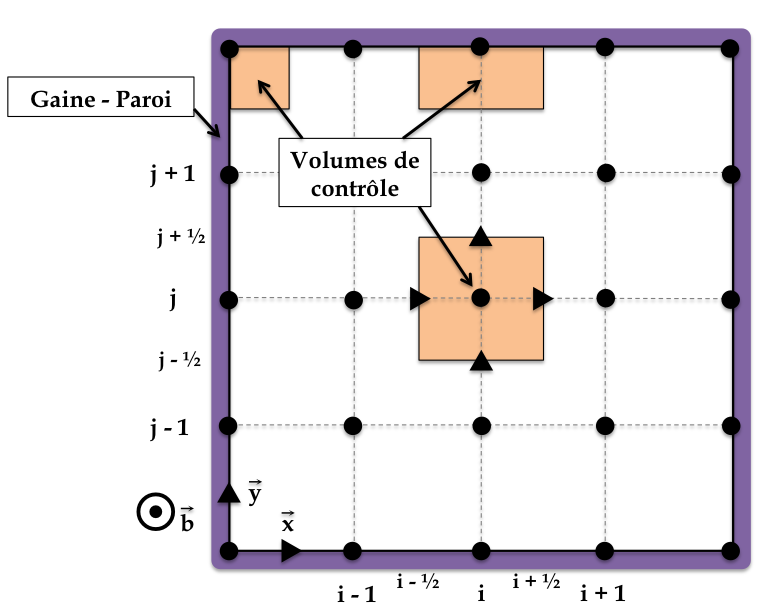
\includegraphics[height=64mm,width=80mm]{figures/3-magnisGrid.png}
{\caption{Schéma du domaine du simulation, entouré d'une gaine
non-collisionnelle.
Les quantités scalaires $n$, $\Phi$ et $T_e$ sont définies aux noeuds et sur les
bords du maillage. Les composantes x et y des champs vectoriels sont
situées entre les noeuds, sur les arêtes des volumes de contrôle, respectivement
au niveau des flêches horizontales et verticales.}
\label{3-maillage}}
\end{figure}

\subsection{Fréquences, termes sources et conditions parallèles}
Avant de résoudre à proprement dit les équations du modèle, MAGNIS
calcule l'ensemble des fréquences : la fréquence de
collision électrons-neutres $\nu_{en}$, ions-neutres $\nu_{in}$ et d'ionisation
$\nu_\text{iz}$. En présence de plusieurs espèces, la fréquence effective, résultat de toutes les
interactions, s'écrit :
\begin{equation*}
\nu_{\alpha s}=n_\alpha\sum_{s\neq\alpha} \frac{m_s}{m_\alpha+m_s}
n_sk^m_{\alpha s}
\end{equation*}

A chaque itération, les coefficients $k^m_{\alpha s}=\left<\sigma^m_{\alpha
s}v_r\right>$, où $\sigma^m_{\alpha
s}$ est la section efficace de l'interaction et $v_r$ la vitesse relative des
particules en collision, sont lus dans des tables en fonction de l'énergie des
particules.
Les valeurs des sections efficaces et des coefficients contenus dans ces tables
sont issues de LXCAT~\parencite{LXCAT}, calculées par des expériences de
swarm~\parencite{Phelps} ou en résolvant directement l'équation de
Bolzmann\parencite{Bolsig}. Un grand
nombre de réactions chimiques peuvent éventuellement être prises en compte.

Le terme source de particule est calculé en fonction de la fréquence
d'ionisation :
\begin{equation*}
S_{\alpha}=n_\alpha n_g k^m_{\alpha_\text{iz}}(T_e)=n_\alpha\nu_{\alpha_\text{iz}}
\end{equation*}

Le terme de perte d'énergie par électron, $\Pi$, est lui aussi fortement
dépendant de la température électronique. Afin de résoudre correctement
l'évolution de la température, le terme est décomposé par une itération
de Newton pour renforcer son influence :
\begin{equation*}
n_e\Pi(T_e^{k+1})=n_e\left(\Pi(T_e^{k})+\frac{\partial\Pi}{\partial
T_e}\left(T_e^{k+1}-T_e^{k}\right)\right)= n_en_g\left(
\frac{\partial k_{\varepsilon}}{\partial T_e}T_e^{k+1}+k_{\varepsilon}\right)
\end{equation*}

avec $k_\varepsilon$ un coefficient de transfert d'énergie (sommé sur 
l'ensemble des processus de collision).

Enfin, les vitesses des particules au niveau des parois sont calculées en
fonction de leur nature isolante, conductrice ou polarisée (les expressions
sont données dans \ref{3-vitessesBord}) puis prisent en compte implicitement
dans les équations de continuités.

\subsection{Expression des vitesses et conservation du courant}
L'un des points clés du modèle tient à la méthode de résolution de l'équation du
mouvement. Ecrivons la comme une équation algébrique
d'inconnue $\mathbf u$, reliant la fréquence caractéristique du transport
$\omega\sim\partial_t$, une fréquence de collision effective $\nu_m$ et la
fréquence cyclotronique $\omega_c$ avec un terme
accélérateur $\mathbf a$ incluant le terme inertiel d'advection :

\begin{equation}
\label{3-eqMvt}
\alpha_\omega\partial_t \mathbf{u} + 
\nu_m\mathbf{u}\pm\omega_{c}\mathbf{b}\times\mathbf{u}=
\mathbf a
\end{equation}

avec 
\begin{equation*}\mathbf a=
-\frac{q\nabla \Phi}{m}-\frac{e\nabla
n T}{m
n}-\alpha_u\mathbf{u}\cdot\nabla\mathbf{u}
\end{equation*}

Les facteurs $\alpha_\omega$ et $\alpha_u$ sont des paramètres numériques qui
permettent de modifier l'influence des termes d'inertie, ou éventuellement de
les négliger ($\alpha_{\omega,u}$=0). Discrétisons temporellement
\eqref{3-eqMvt} en prenant la vitesse implicitement dans les termes
magnétique et collisionnel\footnote{Une récente modification permet de choisir
une résolution implicite du terme
d'inertie $\mathbf{u}\cdot\nabla\mathbf{u}$, rendant le code MAGNIS
full-implicit. Cependant dans ce document, pour des raisons de lisibilité, nous
le laisserons inclus dans la force $\mathbf F$} :

\begin{equation}
\label{3-eqMvtDiscretT}
\delta\left(\mathbf{u}^{k+1}-\mathbf{u}^{k}\right) + 
\nu_m\mathbf{u}^{k+1}\pm\omega_{c}\mathbf{b}\times\mathbf{u}^{k+1}=
\mathbf a
\end{equation}

où $\delta=\alpha_\omega/\Delta t$. En combinant \ref{3-eqMvtDiscretT} et
l'expression de son produit vectoriel par $\mathbf b$, on peut éliminer le
terme de Laplace. La vitesse s'exprime alors comme une somme pondérée du
transport perpendiculaire et du transport croisé :

\begin{equation}
\label{3-eqMvtPonderee}
\mathbf{u}^{k+1}=A\left(\mathbf a + \delta\mathbf{u}^{k}\right)\pm B\mathbf
b\times\left(\mathbf a + \delta\mathbf{u}^{k}\right)
\end{equation}

avec 
\begin{equation*}
\label{3-eqMvtPonderee}
A=\frac{\nu_m+\delta}{(\nu_m+\delta)^2+\omega_c^2}\;\;\;\;\text{et}\;\;\;B=\frac{\omega_c}{(\nu_m+\delta)^2+\omega_c^2}
\end{equation*}

La vitesse telle que définie par \eqref{3-eqMvtPonderee} s'exprime
explicitement en fonction du champ $\mathbf E^k$. 

où $\delta=\alpha_\omega/\Delta t$ prend la place du facteur
usuel $\Delta t\puissance{-1}$ de la dérivée temporelle. Cette opération, qui
peut être vue comme une sous-relaxation de la vitesse électronique en présence
d'un fort champ magnétique, permet  Si $\Delta t\omega_c<$1, il n'y a aucune
substitution,


\subsection{Flux de chaleur et équation d'énergie}

\begin{equation}
S_s(T_e)=n^{k+1}n_gk_{s}^{iz}(T_e)
\end{equation}
où $n_g$ est la densité du gaz et $k_{s}^{iz}$ le coefficient d'ionisation spécifique à l'espèce.
\cite{Hemsworth}

\section{Vérification et validation}

\subsection{Etude de convergence en temps et en espace}
\subsubsection{Densité}
\subsubsection{Potentiel}
\subsubsection{Température}
\subsection{Influence du champ magnétique}
\subsection{Réponses à la température}

%\bibliographystyle{alpha}
%\bibliography{biblio}
\end{refsection}

